%%%%%%%%%%%%%%%%%%%%%%
% Signal selection   %
%%%%%%%%%%%%%%%%%%%%%%

The signal region selection aims for a good discrimination between possible signal processes and
the SM backgrounds. 
As mentioned before, the signals we target with this search have $\cPqb$ tagged jets
and boosted $\W$ bosons in the final state. Therefore, we require, on top of the baseline
selection, the presence of at least one CSV medium $\cPqb$ tagged jet, and at least one $\W$ boson
tagged jet. AK5 jets are used for $\cPqb$ tagging, whereas for $\W$ tagging we use the CA8 jets, as
explained in Section~\ref{sec:boost_wtag}. 
Additionally, we only consider fully-hadronic events and thus select only those events without
loose electrons or muons, and no isolated tracks. 
These selection criteria already reduce the background substantially, but the signal separation
achieved is not yet sufficient. We need an additional handle on the QCD multijet production,
which is the dominant background at this stage. 

Missing transverse energy, \ETm, in multijet events is largely due to jet mismeasurements,
rather than the escape of weakly interacting particles, such as neutrinos or the neutralinos in
signal events. The \VEtmiss vector will, therefore, often be aligned with one of the jets. 
Based on this we can expect that $\Delta\phi_{min}$, the minimum of the angles between \VEtmiss and
the transverse momentum of the leading three jets, will be a good discriminant between multijet
events and events with real \ETm.
\begin{equation}
 \Delta\phi_{min} = \min_{i=1,2,3}{\Delta\phi(\VEtmiss, \ptvec^{\,i})},
\end{equation}
where $i$ runs over the three leading AK5 jets. We require $\Delta\phi_{min} > 0.5$ to suppress
multijet events. The $\Delta\phi_{min}$ distribution, obtained from simulation, before applying this
selection is shown in
Fig.~\ref{fig:boost_signal_mindeltaphi}. The multijet events are clearly gathered in the first few
bins, while the signal extends to much higher values.

\begin{figure}[htbp]
 \centering
 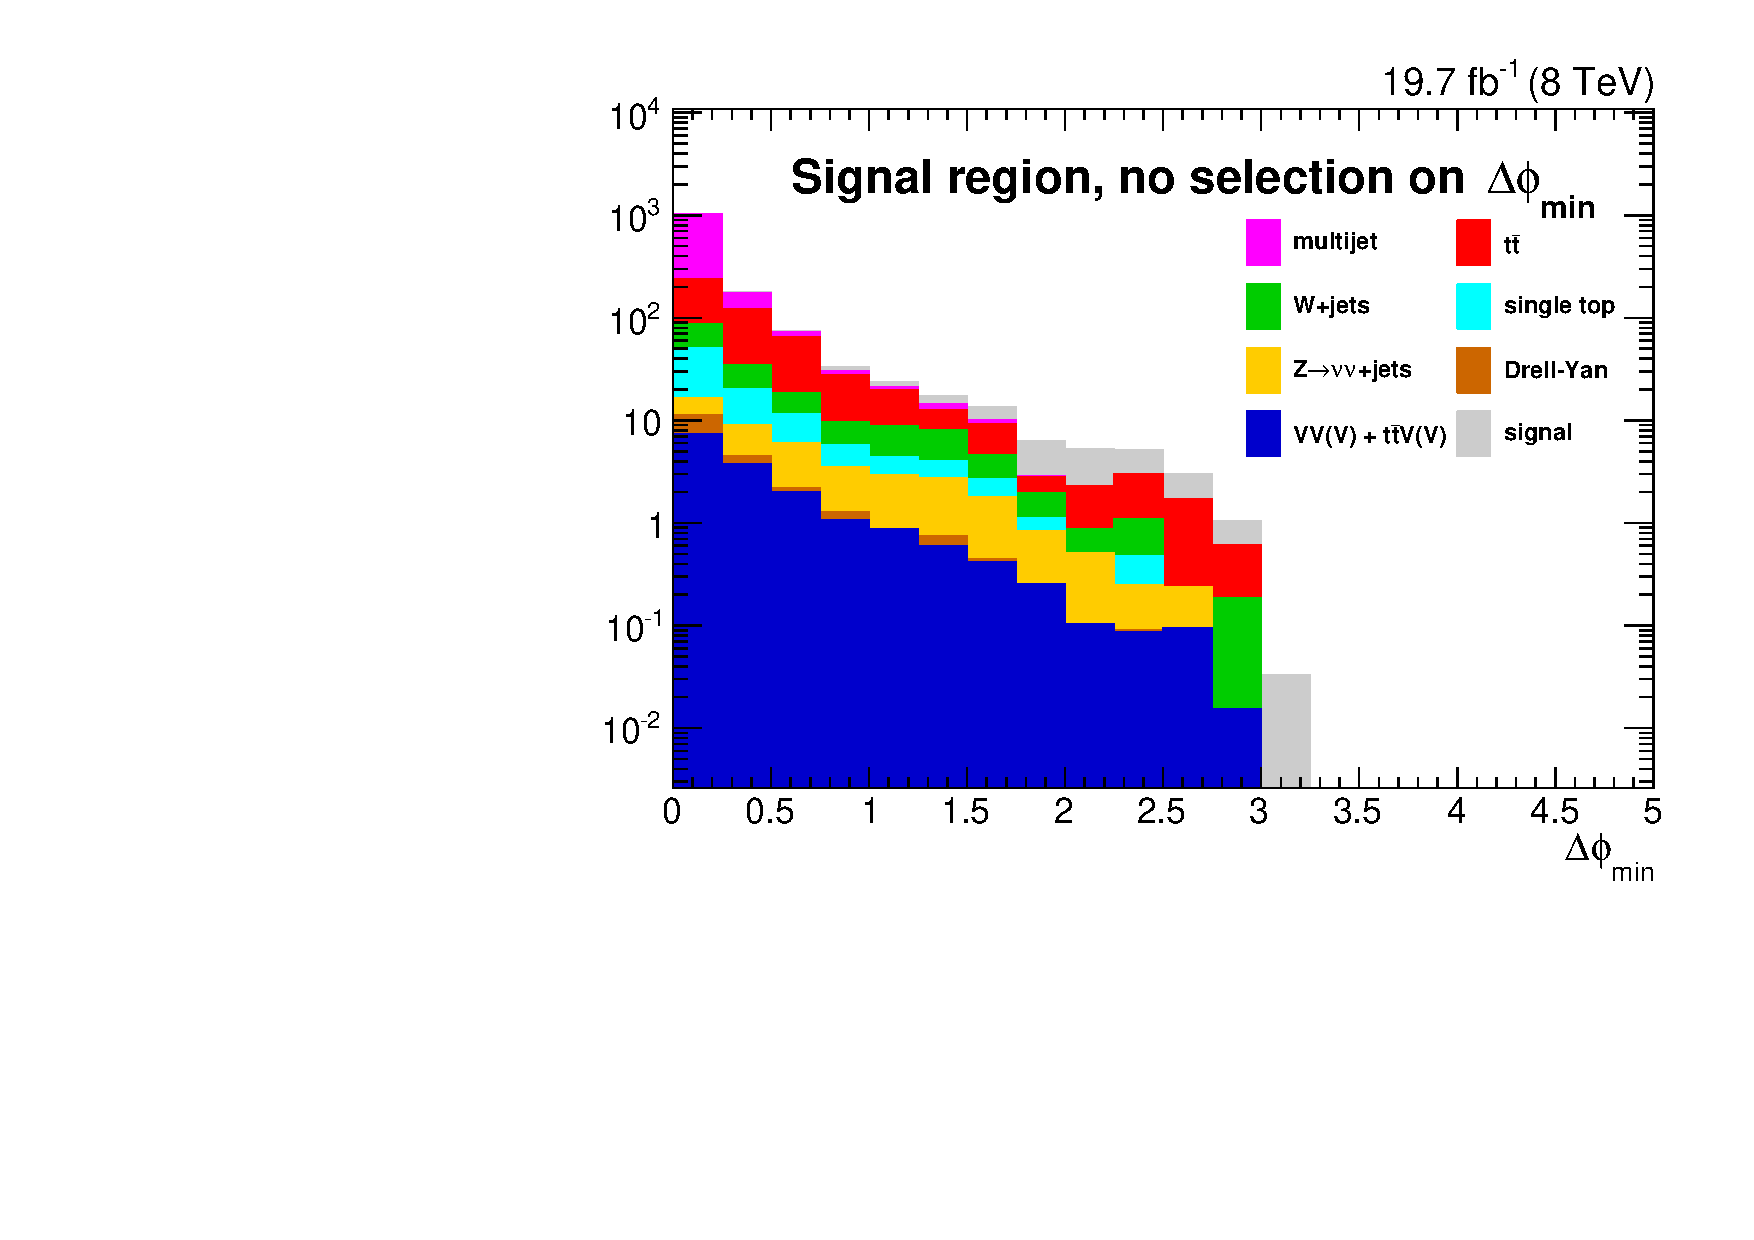
\includegraphics[width=0.8\textwidth]
 {figures/razor_selection/plots/DataMC_minDeltaPhi_g1Mbg1W0Ll_rebin_nodata}
\caption{Simulated $\Delta\phi_{min}$ distribution with all signal region requirements applied
except $\Delta\phi_{min} > 0.5$. QCD multijet events are clearly gathered in the first few bins.
An example signal point is overlaid, and is seen to have a much flatter distribution, extending to
high $\Delta\phi_{min}$ values.
\label{fig:boost_signal_mindeltaphi}}
\end{figure}

A summary of the signal selection is presented in Table~\ref{tab:boost_selection_summary}.
Figure~\ref{fig:boost_signal_dataMC} shows the simulated distributions in the signal region for the
$\mr$ and $\rsq$ variables. The number of events in simulation and data, and the background
composition in percent, are reported in Tables~\ref{tab:cutflow} and \ref{tab:cutflow_summary}, and
Table~\ref{tab:BG_comp_percent}, respectively. 
The signal region is $t\bar{t}$ dominated, with additional contributions from $\W(\rightarrow
\ell\nu)+$jets and multijet processes.
The \pt distribution of the highest \pt tagged $\W$ boson jet in the event is shown in
Fig.~\ref{fig:boost_signal_Wpt_met}, alongside the \ETm distribution.  

\begin{figure}[htbp]
\centering
\includegraphics[width=0.48\textwidth]
{figures/razor_selection/DataMC_MR_g1Mbg1W0Ll_mdPhig0p5_width_nodata_CMS}
~
\includegraphics[width=0.48\textwidth]
{figures/razor_selection/DataMC_R2_g1Mbg1W0Ll_mdPhig0p5_width_nodata_CMS}
\caption{Simulated $\mr$ (left) and $\rsq$ (right) distributions in the signal region. An example
signal point, corresponding to the T1ttcc mass point with $m_{\tilde{g}}
\,{=}\, 1\TeV$, $m_{\stopone} \,{=}\, 325\GeV$ and $m_{\lsp} \,{=}\, 300\GeV$, is
stacked on top of the background processes. The bin entries are normalized proportional to the bin
width.  
\label{fig:boost_signal_dataMC}}
\end{figure}

\begin{figure}[htbp]
\centering
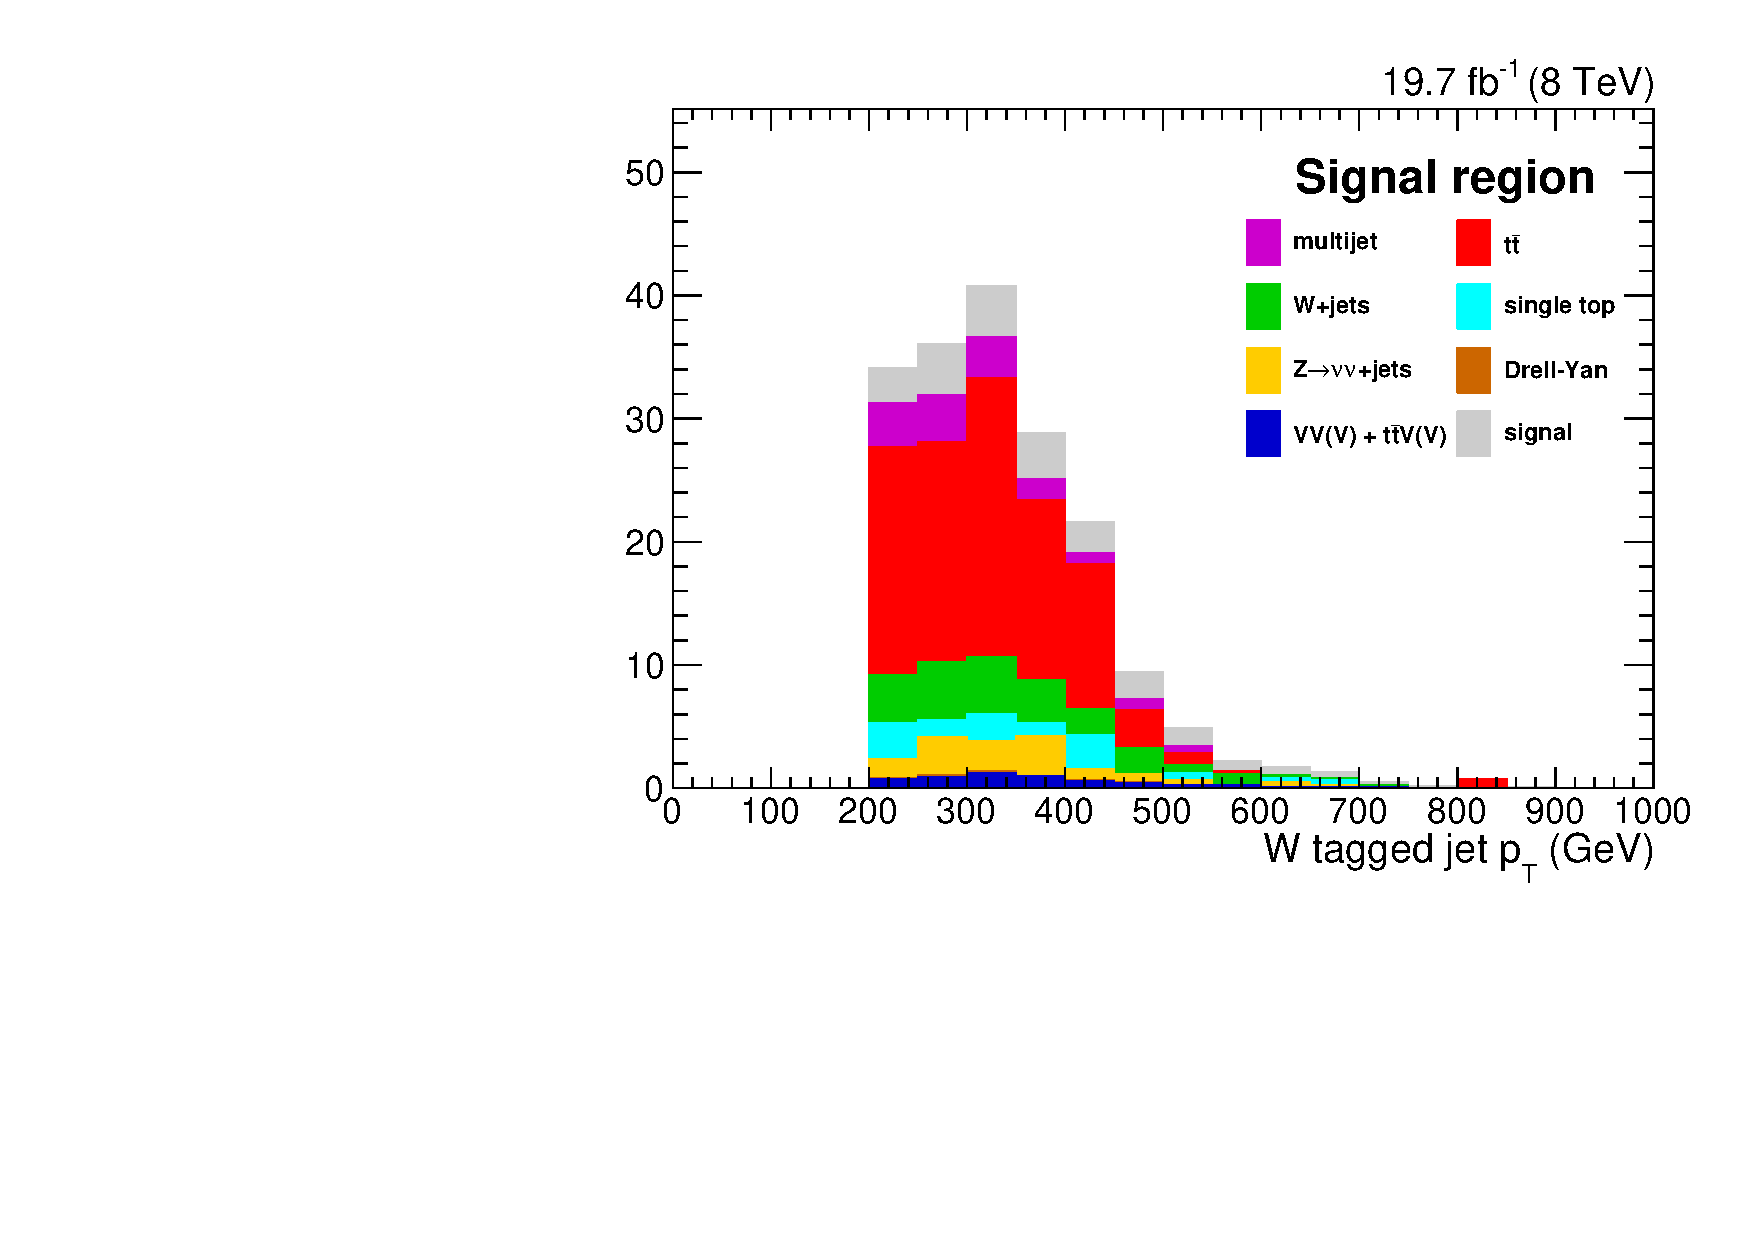
\includegraphics[width=0.48\textwidth]
{figures/razor_selection/plots/DataMC_Wpt_g1Mbg1W0Ll_mdPhig0p5_nodata}
~
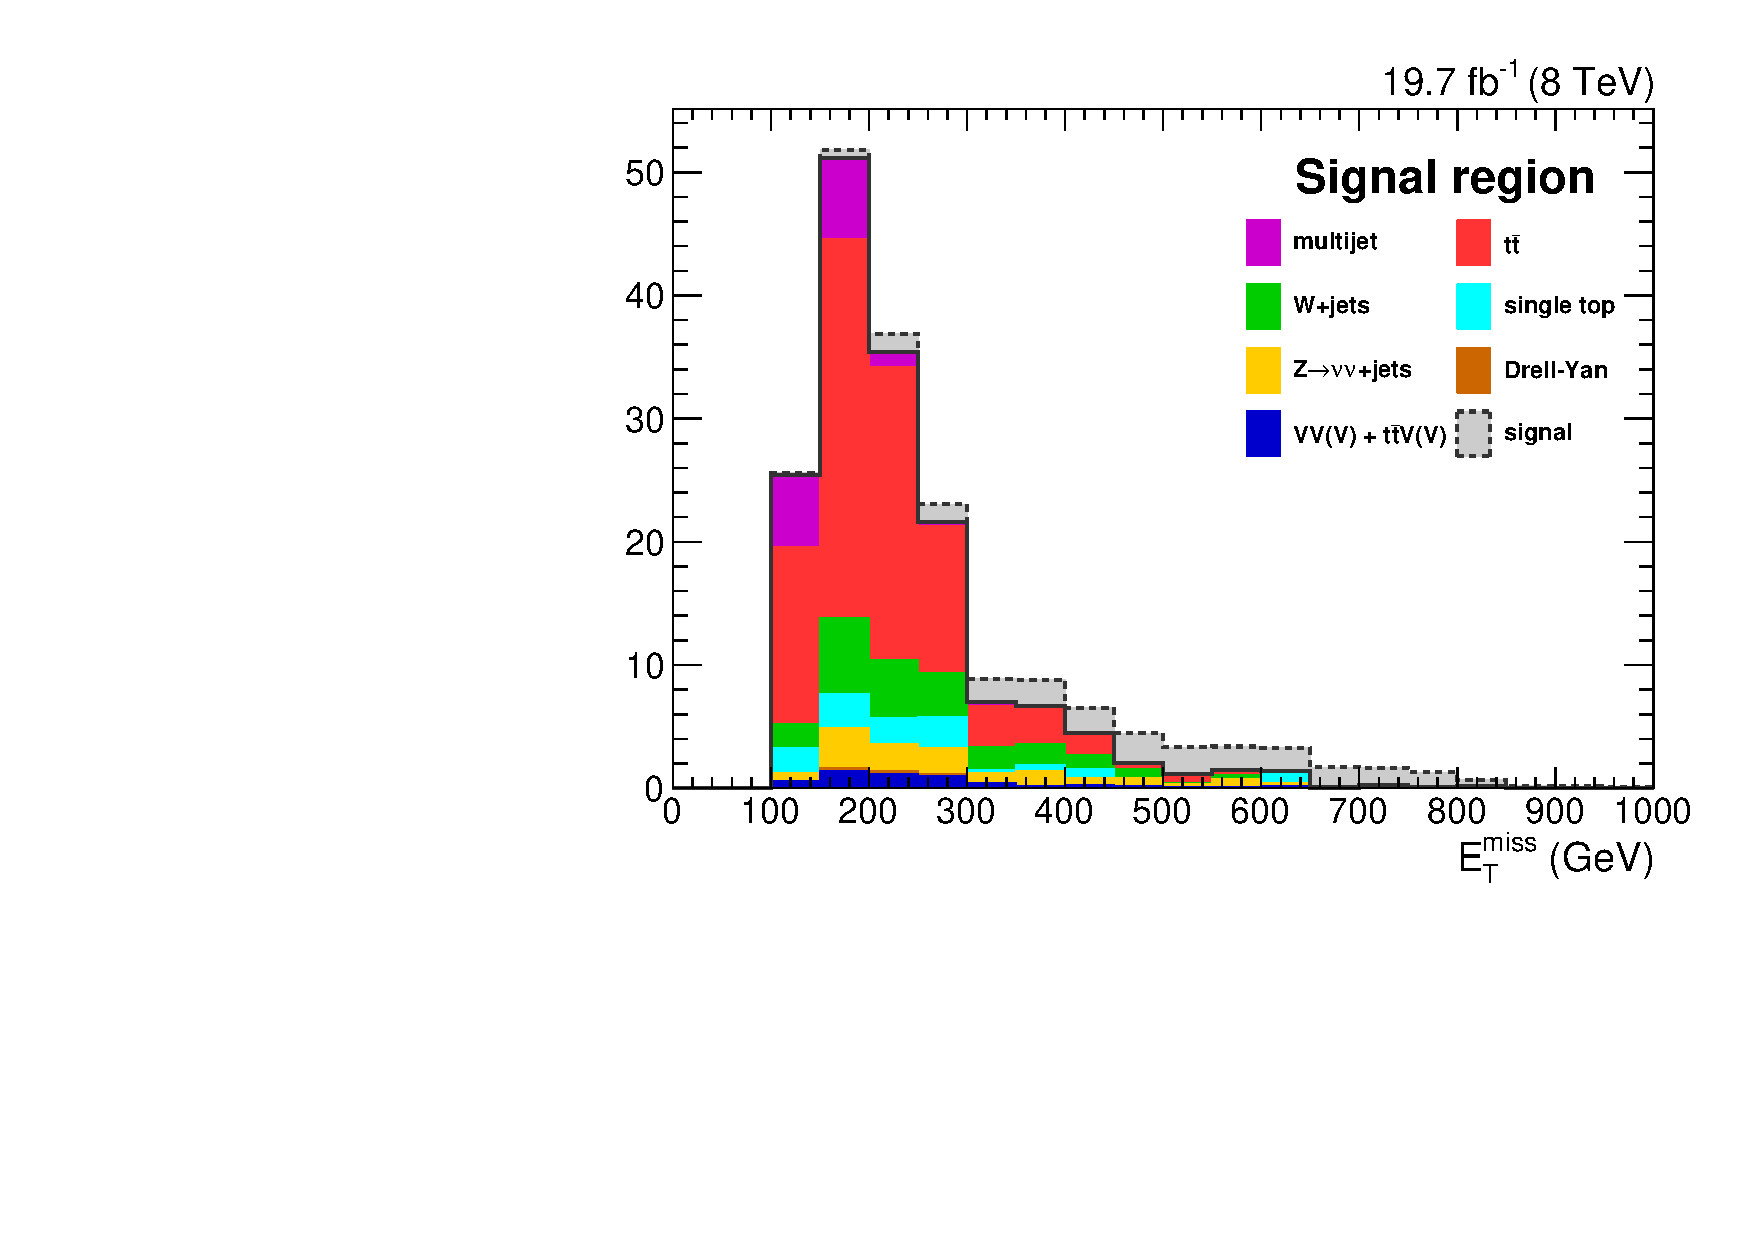
\includegraphics[width=0.48\textwidth]
{figures/razor_selection/plots/DataMC_met_g1Mbg1W0Ll_mdPhig0p5_nodata}
\caption{Simulated $\W$ tagged jet $\pt$ (left) and $\ETm$ (right) distributions in the signal
region. An example signal point, corresponding to the T1ttcc mass point with $m_{\tilde{g}}
\,{=}\, 1\TeV$, $m_{\stopone} \,{=}\, 325\GeV$ and $m_{\lsp} \,{=}\, 300\GeV$, is
stacked on top of the background processes. 
\label{fig:boost_signal_Wpt_met}}
\end{figure}



% In figures~\ref{fig:DataMC_SignalRegion_MR_R2_mdphig0p5} and \ref{fig:DataMC_SignalRegion_mdphig0p5}
% we show a Data/MC comparison for various quantities for the signal region with $\Delta\phi_{min} >
% 0.5$. 
% Please note that these plots are for illustration purposes only. 
% We will predict the background using data control regions and only use the simulation for
% translation factors between those control regions and the signal region (see further). We stress in
% particular that the QCD multijet MC is underpredicting what we see in data.
% 
% \begin{figure}[p]
%  \includegraphics[width=0.49\textwidth]{figures/DataMC/DataMC_njets_g1Mbg1W0Ll_mdPhig0p5}
%  \includegraphics[width=0.49\textwidth]{figures/DataMC/DataMC_nbjets_g1Mbg1W0Ll_mdPhig0p5}
% 
%  \includegraphics[width=0.49\textwidth]{figures/DataMC/DataMC_met_g1Mbg1W0Ll_mdPhig0p5}
%  \includegraphics[width=0.49\textwidth]{figures/DataMC/DataMC_jet1pt_g1Mbg1W0Ll_mdPhig0p5}
% 
%  \includegraphics[width=0.49\textwidth]{figures/DataMC/DataMC_jet2pt_g1Mbg1W0Ll_mdPhig0p5}
%  \includegraphics[width=0.49\textwidth]{figures/DataMC/DataMC_jet3pt_g1Mbg1W0Ll_mdPhig0p5}
% \caption{For illustration only: Data/MC comparison plot of various event quantities in the signal
% region requiring $\Delta\phi_{min} > 0.5$: 
% [top] jet multiplicity (left) and b-tagged jet multiplicity (right);
% [middle] missing transverse energy (left) and \pt of the highest \pt jet (right);
% [bottom] \pt of the second (left) and third (right) highest \pt jet. 
% \label{fig:DataMC_SignalRegion_mdphig0p5}}
% \end{figure}
% 
% \begin{figure}[htbp]
%  \includegraphics[width=0.49\textwidth]{figures/DataMC/DataMC_Wpt_g1Mbg1W0Ll_mdPhig0p5}
%  \includegraphics[width=0.49\textwidth]{figures/Shapes/comparison_Wpt}
% \caption{For illustration only: [left] Data/MC comparison plot of $\pt(W)$ in the signal region
% requiring $\Delta\phi_{min} > 0.5$.
% [right] Comparison of the $\pt(W)$ distribution for signal and total background. Both distributions
% are normalized to unit area.
% \label{fig:Wpt_SignalRegion}}
% \end{figure}
% 
